\documentclass[12pt, a4paper, polish, openany]{book}
\usepackage{styl-notatek}
\begin{document}
\onehalfspacing
\begin{titlepage} 
    \begin{center}
         \begin{figure}[h]
            \centering
            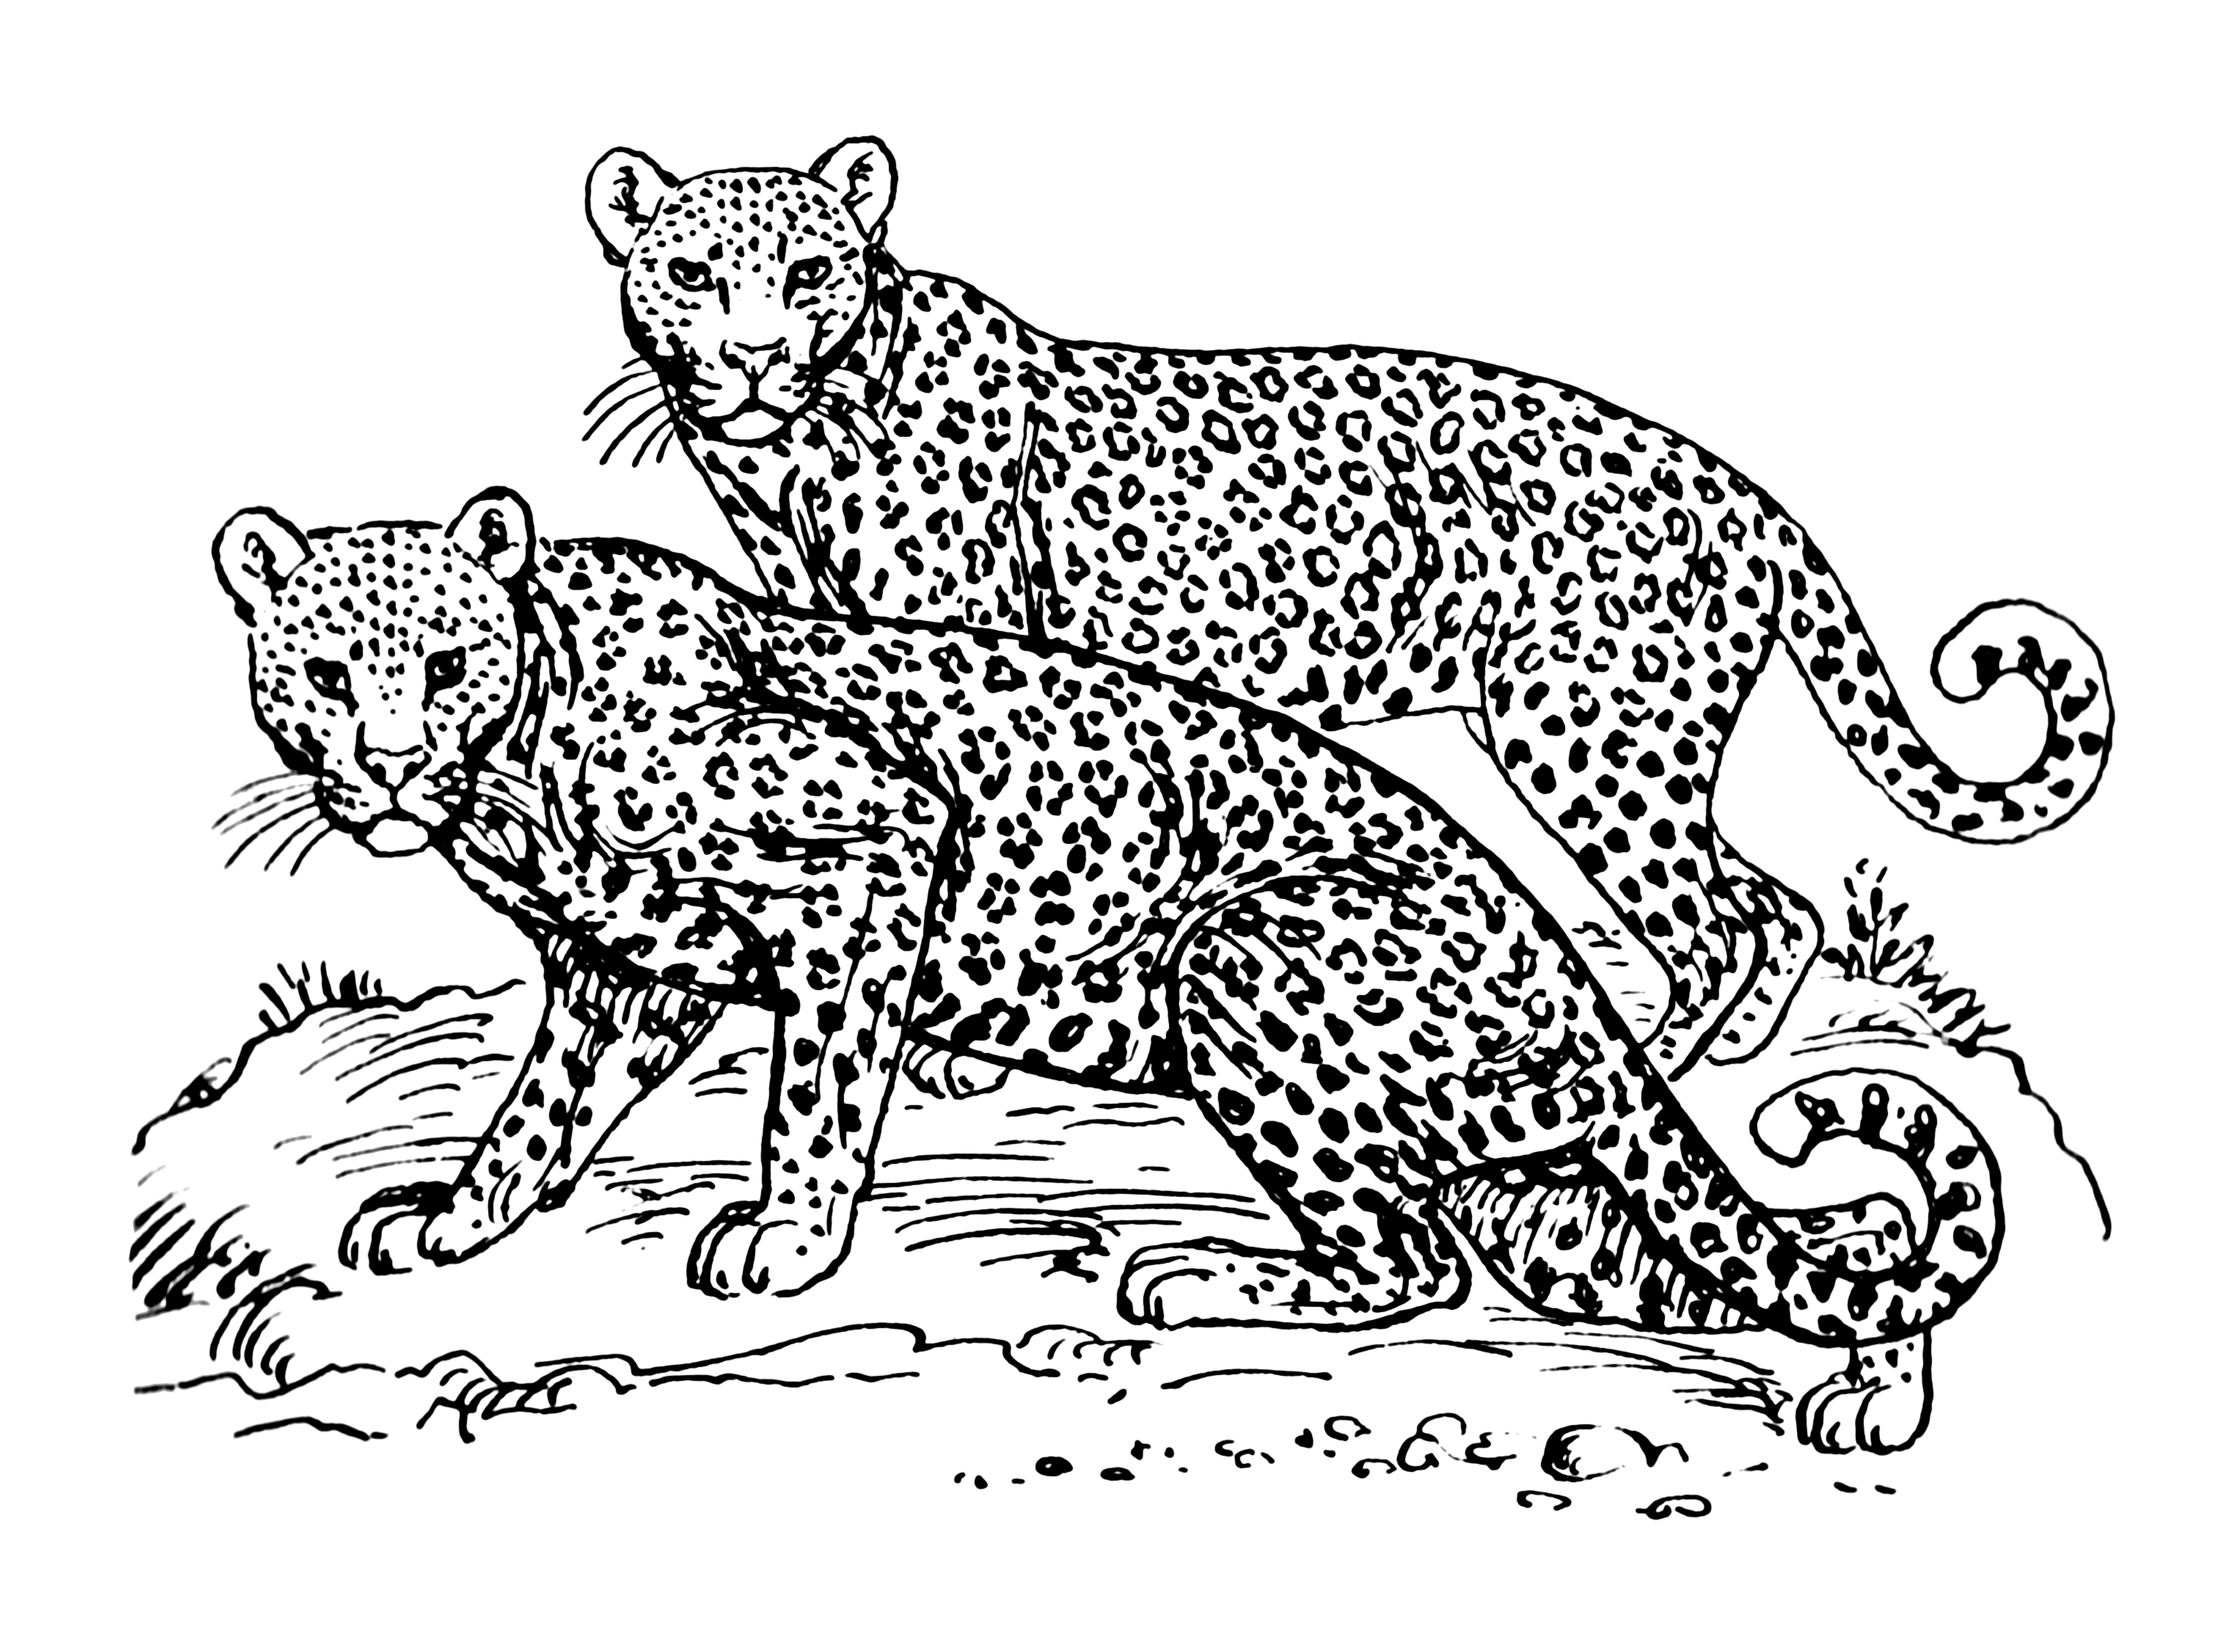
\includegraphics[]{img/pumy.png}
           
        \end{figure}
        
        \Huge
        \textbf{\textsc{Metody Probabilistyczne \\ w Uczeniu Maszynowym}}
        
        \vspace{0.5cm}
        \Large
        \textsc{Zagadnienia Egzaminacyjne}
        \line(1,0){330}
        
        \normalsize
        
        \vspace{1cm}
        \textit{,,Gdzie błąd?''}
        \vspace{1cm}

        \textit{\textsc{Popełnione przez}}\\
        \vspace{5mm}
  
        \textbf{\textsc{Załatany Ponton}}
 
        \vfill

        Kraków \\
        Anno Domini 2023
    \end{center}
\end{titlepage}
\fancyhead[L]{\textbf{\textit{SO}}}
\fancyhead[C]{\thepage}
\fancyhead[R]{
\includegraphics[width=1cm]{tcs.png}}
\tableofcontents
\section*{Licencja}
    \begin{figure}[h]
    	\begin{minipage}[c]{0.25\textwidth}
    		
\includegraphics[width=0.7\textwidth]{licencja.png}
    	\end{minipage}\hfill
    	\begin{minipage}[c]{0.75\textwidth}
    		\caption*{
    			Ten utwór jest dostępny na 
    			\href{https://creativecommons.org/licenses/by-sa/4.0/}{licencji Creative Commons Uznanie autorstwa
    			na tych samych warunkach 4.0 Międzynarodowe.}
    		}
    	\end{minipage}
    \end{figure}

\chapter{POSIX}
\section{Główne zadania systemu operacyjnego}
\begin{itemize}
  \item obsługa plików
  \item poziom abstrakcji nad handlerem, tak aby nie dawać użytkownikowi bezpośredniego dostępu do hardware'u
\end{itemize}
\section{Nalot, cechy POSIXa}
\begin{itemize}
  \item Jest tylko specyfikacją, a nie konkretną implementacją
  \item Oparty na C
  \item Nie ma superużytkownika ani administracji systemu
  \item Łatwy w implementacji (relatywnie)
  \item Historycznie jedynie niewielkie znaczące zmiany
\end{itemize}
\section{Procesy}
\textbf{Proces} - program w trakcie wykonywania
\section{Wywołania systemowe}
Wywołania systemowe stanowią interfejs między wykonywanym programem a (posiadającym zwykle wyższe uprawnienia) jądrem systemu operacyjnego.\\
\textbf{Przykłady wywołań systemowych (syscalli)}
\begin{itemize}
  \item exit - kończy proces i opróżnia wszystkie bufory oraz sprząta to, czego wymaga biblioteka standardowa, \_exit po prostu zakańcza proces
  \item fork - tworzy nowy proces równoległy z aktualnym, wykonujący ten sam kod, ma on jednak unikalny pid, inny ppid, i własną kopię deskryptorów rodzica oraz zablokowane te same sygnały
  \item exec* rodzinka syscalli - \ref{execve}
  \item wait - blokuje proces, póki wszystkie dzieci żyją albo otrzymano sygnał
  \item kill \ref{kill}
  \item waitpid - blokuje proces, dopóki proces o podanym pidzie się nie skończy. Dozwolone jest czekanie tylko na swoje dzieci.
\end{itemize}
\subsection{Syscall execve}
\label{execve}
Podmienia wykonywany przez proces program, np. po zforkowaniu, aby dziecko wykonywało inny kod. Podajemy mu ścieżkę do binarki lub, jeśli coś jest dodane do kontekstu, nazwę. \\
\textbf{Efekty uboczne:}
\begin{itemize}
  \item \textbf{domyślnie deskryptory plików pozostają otwarte!}
  \item przekierowania sygnałów do handlerów są zresetowane
  \item mapowania pamięci nie są zachowywane, są odmapowywane
  \item deskryptory do do POSIXowych wiadomości systemowych są zamykane.
  \item zamykane są wszystkie POSIXowe semafory
  \item wszystkie pozostałe wątki procesu są zamykane
\end{itemize}

\section{Deskryptory plików}
Deskryptory plików to unikalne dla procesów dodatnie inty używane do identyfikacji otwartych plików. Przyjmują wartości od 0 do OPEN\_MAX, w POSIXie standardowo jest to max 16 otwartch plików. Co ciekawe, plik może być zreferowany przez dwa różne deskryptory, ale jeden deskryptor zawsze wskazuje na tylko jeden plik, czyli pomiędzy deskryptorami a open file description jest relacja many-to-one. Jedyną znaną nam flagą deskryptora pliku jest FD\_CLOEXEC. \\\\
Domyślnie otwarte są deskryptory: 0 - stdin, 1 - stdout, 2 - stderr.
\subsection{Otwieranie nowych deskryptorów}
Nowe deskryptory otwieramy przy pomocy syscala \textbf{open}, który przyjmuje ścieżkę do pliku oraz flagi:
\begin{itemize}
  \item O\_RDONLY, otwarcie tylko do czytania
  \item O\_WRONLY, otwarcie tylko do pisania
  \item O\_RDWR, otwarcie do czytania i pisania
  \item O\_NONBLOCK, wyłącza domyślne blokowanie 
  \item O\_APPEND, każdy write pisze na końcu pliku
  \item O\_CREAT, stwórz plik, jeśli nie istnieje
  \item O\_EXCL, wyrzuca błąd kiedy plik już istniał
\end{itemize}
Aby połączyć dwie flagi używamy logicznego lub \xrightarrow[]{} |, np. $\;$ (O\_CREAT $\;$ | $\;$ $\_EXCL)$. \\
Funkcja open tworzy nowy \textbf{open file description}, w której przechowywane są flagi.
\subsection{Czytanie z pliku}
Czytamy przy pomocy syscalla \textbf{read}, który przyjmuje deskryptor, wskaźnik gdzie zapisać dane i liczbę byte'ów do przeczytania. Zwraca liczbę byte'ów, które udało mu się przeczytać lub 0, jeśli przytrafi się EOF.
\subsection{Pisanie do pliku}
Piszemy do pliku przy pomocy syscalla \textbf{write}, który przyjmuje deskryptor, wskaźnik na dane do zapisania i liczbę byte'ów do zapisania. Zwraca liczbę byte'ów, które udało mu się zapisać.\\\\
Domyślnie read i write są blokujące. Jeśli zostaną przerwanę przez jakiś sygnał zanim przeczytają / zapiszą cokolwiek to zwrócą -1 i ustawią errno na EINTR. Jeśli przeczytają trochę danych, ale niekoniecznie tyle, o ile prosiliśmy, to zwrócą rozmiar opracowanych danych i się przerwą.
\subsection{Seek}
Możemy zmienić aktualną pozycje w pliku bez czytania za pomocą \textbf{seek}, który przyjmuje deskryptor, $d$ liczbę byteów o którą mamy się przesunąć i flagę, która ustala, odkąd liczymy przesunięcie: \textbf{SEEK\_SET} przesuwa na $d$ pozycji względem początku pliku, \textbf{SEEK\_CUR} względem aktualnej pozycji, a \textbf{SEEK\_END} względem końca pliku. \\
Przykład
\begin{verbatim}
  int fd = open("foo", O_RDWR | O_CREAT | O_TRUNC, S_IRUSR | S_IWUSR);
  lseek(fd, 10000000000L , SEEK_CUR ); // ˜10GB
  write(fd, "a", 1);
  close(fd);
\end{verbatim}
Mimo że plik będzie miał rozmiar 1000000001, to będzie wyświetlane tylko "a".
\section{Pipe'y}
Pipe'y to kanały komunikacji, które pozwalają przesyłać informacje pomiędzy procesami. 
\begin{verbatim}
  int pipe(int fildes[2])
\end{verbatim}
Pipe'a tworzymy, podając syscallowi \textbf{pipe} dwuelementową tablicę intów. Syscall stworzy pipe i ustawi fildes[0] na koniec do czytania (read descriptor) i fildes[1] na koniec do pisania (write descriptor). Dane zapisane do write końca są buforowane przez kernel, póki nie zostaną przeczytane z read końca. Pipe ma maksymalny rozmiar, jeśli jest dużo nieprzeczytanych danych, to write się zablokuje.
\subsection{FIFO - named pipe'y}
Nazwane pipe'y działają trochę jak pipe'y, trochę jak pliki. Tworzymy je syscallami mknod lub mkfifo, przy czym mknod jest zarezerwowany tylko dla superużytkownika. Tworząc je, musimy podać ścieżkę, pod którą będą się znajdować, tak aby procesy bez wcześniejszego porozumiewania się mogły je znaleźć, zwykle najlepiej je tworzyć w folderze $/tmp/$. Potem otwieramy je jak pliki i czytamy z nich lub piszemy do nich jak do zwyczajnych pipe'ów.
\begin{verbatim}
  int mknod(const char *path, mode_t mode, dev_t dev)
  int mkfifo(const char *path, mode_t mode)
\end{verbatim}
Otwieranie nazwanego pipe'a do pisania (O\_WRONLY), w przeciwieństwie do otwierania go do czytania (O\_RDONLY), które jest blokujące, nie powiedzie się, jeśli po drugiej stronie nie ma czytelnika (przynajmniej na linuxie) i zwróci -1.
\subsection{Uwagi co do równoległego czytania}
Równoległe odczyty z pipe'ów, fifo i terminalu to działania niezdefiniowane. Może zadziała, a może nie.\\
Operacje I/O powinny być atomowe, czyli wszystkie bajty z danej operacji powinny być obok siebie, nie przeplecione bajtami z innych operacji. Dla Pipe'ów, FIFO i plików to zwykle działa, ale terminale są prawie zawsze wyłączone od tej zasady, tam nie można na tym polegać.\\
Write'y o rozmiarze mniejszym niż bufor pipe'a nie powinny być przeplecione write'ami z innych pipe'ów, ale jeśli są większe nie ma takiej gwarancji.
\subsection{fcntl}
fcntl pozwala wykonać komendę podaną w argumencie cmd na deskryptorze pliku
\begin{verbatim}
  int fcntl(int fd, int cmd, [data])
\end{verbatim}
\section{Sygnały}
Sygnały informują o asynchronicznym zdarzeniu, często o błędzie.
\subsection{Źródła sygnałów}
\begin{enumerate}
  \item Ctrl-C wysyła \textbf{SIGINT} do wszystkich procesów z foregroundu
  \item Ctrl-$\backslash$ wysyła \textbf{SIQUIT} do wszystkich procesów z foregroundu
  \item Dzielenie przez 0 powoduje wysłanie sygnału \textbf{SIGFPE} do procesu
  \item Procesy mogą wysyłać sygnały poprzez syscall kill \ref{kill}
\end{enumerate}
\\
Do adresata nie docierają sygnały $SIGKILL$ i $SIGSTOP$, odbiera je kernel i odpowiednio zabija / pauzuje proces.
\subsection{Ważne sygnały}
\begin{itemize}
  \item \textbf{SIGINT} - żądanie przerwania od użytkownika
  \item \textbf{SIGKILL} - absolutne zakończenie procesu bez sprzątania
  \item \textbf{SIGTERM} - domyślny sygnał wysyłany przez funkcję kill
  \item \textbf{SIGSTOP}
  \item \textbf{SIGILL}
  \item \textbf{SIGALRM} - sygnał wykorzystywany w syscallu alarm
  \item \textbf{SIGCHLD}
\end{itemize}
Sygnały SIGSTOP i SIGKILL nie mogą być ignorowane ani blokowane.
SIGTERM, SIGINT i SIGQUIT mają jako domyślną obsługę zakończenie procesu, przy czym SIGTERM być może trochę posprząta, zanim całkowicie zakończy proces, a SIGQUIT zrobi core dump. \\
Prośba o wysłanie SIGALARM anuluje wszystkie poprzednie alarmy. Podanie 0 jako arguemnt do funkcji alarm anuluje wszystkie alarmy. Przenoszą się przez execve, ale nie są dziedziczone przez procesy stworzone przez fork.

\subsection{Syscall kill}
\label{kill}
Wysyła sygnał do danego procesu o tym samym ID użytkownika. 
\begin{verbatim}
  int kill(pid_t pid, int sig);
\end{verbatim}
\textbf{Adresaci}:
\begin{itemize}
  \item pid$>$0 proces, którego id jest równe pid
  \item pid=0 procesy z tej samej grupy co wysyłający
  \item pid=-1 wszystkie procesy (do których można wysyłać)
  \item pid$<$ -1 wszystkie procesy z grupy o ID równym $|$pid$|$
\end{itemize}
\\
Syscall raise pozwala wysłać sygnał do samego siebie
\begin{verbatim}
  int raise(int sig);
\end{verbatim}
\subsection{Przekierowywanie sygnałów}
\subsubsection{Signal - ISO C}
Signal pozwala nam zmienić domyślne działanie sygnału. Nie jest częścią POSIXa, jest częścią standardu C.
\begin{verbatim}
  void (*signal(int signo, void (*func)(int)))(int);
\end{verbatim}
Jako drugi argument możemy podać wskaźnik do funkcji, która ma obsługiwać sygnał albo ustawić flagę na \textbf{SIG\_IGN}, co pozwala na całkowite zignorowanie sygnału. Możemy też przywrócić domyślną obsługę poprzez ustawienie flagi na \textbf{SIG\_DFL}. Funkcja signal ustawia obsługę sygnału tylko na jeden raz, a później przywracana jest domyślna.
\subsubsection{Sigaction - POSIX}
Sigaction także pozwala nam zmienić domyślne działanie sygnału, jest zdefiniowany w POSIXie.
\begin{verbatim}
  int sigaction(int sig, const struct sigaction *restrict act,
          struct sigaction *restrict oact);
\end{verbatim}
Struktura sigaction jest zdefiniowana jako
\begin{verbatim}
  struct sigaction {
    void    (*sa_handler)(int); // wskaźnik do funckji, która
          będzie obsługiwać sygnał lub SIG_IGN / SIG_DFL
    void    (*sa_sigaction)(int, siginfo_t *, void *); 
    sigset_t  sa_mask; // zbiór sygnałów, które chcemy zablokować
    int    sa_flags; // flagi
    void    (*sa_restorer)(void);
  };
\end{verbatim}

\textbf{Flagi:}
\begin{itemize}
  \item \textbf{SA\_SIGINFO} w sigaction pozwala nam na uzyskanie dodatkowych informacji o procesie.\\
  Jeśli flaga SA\_SIGINFO jest ustawiona, to musimy zdefiniować funkcję obsługującą sygnały jako:
  \begin{verbatim}
  void func(int signo, siginfo_t *info, void *context);
  \end{verbatim}
  \item \textbf{SA\_RESTART}, po jej ustawieniu, jeśli odebranie sygnału przerwało jakąś funkcje blokującą, to wznowi on działanie po obsłudze procesu, zamiast się zakończyć z błędem. Przydatne np. do reada i write'a.
  \item \textbf{SA\_NOCLDSTOP} wyłącza generowanie sygnałów SIGCHLD, kiedy proces dziecko się zakończy. Przydatne, gdyż ustawienie wprost obsługi SIGCHLD na SIG\_IGN jest niezdefiniowane w POSIXie i mogą się dziać złe rzeczy. W Linuxie jednak można ignorować SIGCHLD, aby zapobiec powstawaniu procesów zombie.
\end{itemize}
\textbf{UWAGA!} takie same sygnały w POSIXie nie są kolejkowane, to znaczy kiedy dostaniemy wiele takich samych sygnałów na raz to nie ma gwarancji, że handler wywoła się tyle razy, ile sygnałów dostaliśmy. Jeśli jednak dostaliśmy wiele różnych sygnałów, to mamy gwarancję, że handler dla każdego typu sygnału wykona się co najmniej raz.
\subsection{sigprocmask}
sigprocmask pozwala nam zablokowywać/odblokowywać procesy zgodnie z podaną maską.
\begin{verbatim}
  int sigprocmask(int mode, const sigset_t *restrict set,
    sigset_t *restrict oset);
\end{verbatim}
\textbf{Dostępne tryby}
\begin{itemize}
  \item SIG\_BLOCK zablokuj podane sygnały
  \item SIG\_SETMASK zbiór zablokowanych sygnałów ma być podanym zbiorem (wcześniejsze ustawienia są zapominane)
  \item SIG\_UNBLOCK odblokuj podane sygnały (nawet jeśli były zablokowane przed zmianami, nie przywraca poprzedniego stanu)
\end{itemize}
\subsection{sigsuspend}
Zmienia maskę na podaną, po czym zawiesza się aż do otrzymania niezablokowanego sygnału, po czym przywraca poprzednią maskę.
\begin{verbatim}
  int sigsuspend(const sigset_t *sigmask);
\end{verbatim}
\subsection{sigpending}
sigpending zapisuje w podanym sigsecie wszystkie sygnały, które zostały zablokowane i oczekują na wywołanie, przydatne gdy chwilowo musieliśmy zablokować sygnały podczas wykonywania krytycznych operacji
\begin{verbatim}
  int sigpending(sigset_t *set);
\end{verbatim}
\subsection{Czekanie na wiele deskryptorów na raz}
\subsubsection{select}
select pozwala nam na czekanie na wiele deskryptorów na raz, aż będzie można do nich pisać / czytać. Podajemy tablicę deskryptorów do readfs / writedfs / errordfs w zależności od rodzaju. Później możemy sprawdzić, czy konkretny deskryptor jest gotowy przez FD\_ISSET. Gotowość niestety może czasami okazać się sytuacją, kiedy po drugiej stronie nie ma nikogo... Jeśli działa, to trzeba go resetować przez FD\_CLEAR w każdym wywołaniu, bo zmienia on readfs. 
\begin{verbatim}
int select(int nfds, fd_set *restrict readfds,
  fd_set *restrict writefds, fd_set *restrict errorfds,
  struct timeval *restrict timeout);
  void FD_CLR(int fd, fd_set *fdset);
  int FD_ISSET(int fd, fd_set *fdset);
  void FD_SET(int fd, fd_set *fdset);
  void FD_ZERO(fd_set *fdset);
\end{verbatim}
\subsubsection{pselect}
to samo co select, ale ma mniej ograniczeń i można mu podać dodatkowo maskę sygnałów, które chcemy zablokować podczas czekania i nie trzeba go resetować.
\begin{verbatim}
  int pselect(int nfds, fd_set *restrict readfds,
    fd_set *restrict writefds, fd_set *restrict errorfds,
    const struct timespec *restrict timeout,
    const sigset_t *restrict sigmask);
\end{verbatim}
\subsubsection{poll}
\newpage
\chapter{OS-internals}
\section{Multiprogramming}
\section{Scheduler}
Scheduler zarządza dostępem procesów do czasu procesora, zatrzymując co niektóre i wznawiając inne.
\subsection{Schedulery czasu rzeczywistego}
Procesy mają przypisane priorytety i pierwszy wykona się ten o najmniejszym priorytecie spośród gotowych.
\subsubsection{Round Robin}
Każdy proces dostaje kwant czasu i jest ustawiony w kolejce. Proces może działać tak na jak długo wystarczy mu kwantu, a kiedy go zużyje trafia na koniec kolejki i otrzymuje nowy. Jeśli proces zablokuje się w oczekiwaniu na zasoby przed zużyciem kwantu, to po odblokowaniu trafia na początek kolejki z czasem, jaki mu pozostał.\\\\
Bardzo istotny jest dobór wielkości kwantu, za duży powoduje, że system ma zbyt długi czas reakcji, zbyt mały powoduje dużo zmarnowanej pracy na zmiany kontekstu. Zwykle używa się między 20-50ms.
\subsubsection{Priority Scheduling}
Bazuje na round robin, kwanty czasu zależą od priorytetu, procesy o niższym priorytecie mają pierwszeństwo. 
\subsubsection{Guaranteed Scheduling / Fair share scheduling}
Każdy proces ma zagwarantowane x\% procesora, scheduler dobiera procesy tak, aby dopełnić zobowiązania.
\subsubsection{Lottery Scheduling}
Każdy proces dostaje kilka żetonów z puli. Scheduler losowo dobiera żeton i przydziela procesor jego właścicielowi. Współpracujące procesy mogą sobie przekazywać żetony.
\subsubsection{A jak to jest w minixie?}
W minixie używany jest priority scheduling z dodatkową degracją (zwiększeniem) priorytetu. Procesy użytkownika zwiększają swój priorytet, jeśli zużyły cały kwant i dwa razy z rzędu dostały procesor, zmniejszają w przeciwnym przypadku.
\subsection{Przerwania}
Scheduler pracuje podczas przerwań, w tym w szczególności przerwań zegarowych. Im więcej przerwań zegarowych, tym efektywniej można zarządzać pracą procesów, ale z drugiej strony tym więcej czasu procesora jest wykorzystane przez scheduler i na zmianę kontekstu. W minixie jest 60 przerwań na sekundę
\subsection{Wątki}
Każdy proces posiada przynajmniej jeden wątek. Procesy mają oddzielne przestrzenie adresowe, a wątki mogą je współdzielić. Wątki jednego procesu mają wspólne między innymi:
\begin{itemize}
  \item Wskaźnik do segmentu tekstowego (PM)
  \item Wskaźnik do segmentu danych (PM)
  \item Wskaźnik do segmentu bss (PM)
  \item Wskaźnik do stosu (K)
  \item Stan procesu (K)
  \item Licznik programu (K)
\end{itemize}
K - kernel, PM - process management
\subsection{Zachowanie Procesów}
Dzielimy procesy na kategorie i każda z nich jest traktowana inaczej. Scheduler dba o to, żeby podobne procesy były podobnie traktowane i utrzymuje równe obciążenie wszystkich części systemu.
\begin{itemize}
  \item \textbf{Interaktywne} - Mają najwyższy priorytet. Scheduler stara się, aby szybko reagowały na input. W zależności od czasu trwania zadania scheduler pozwala sobie na opóźnienie reakcji (nie zrobi nikomu różnicy, jeśli ls wypisze coś w 0.05 sekundy zamiast 0.01).
  \item \textbf{Wsadowe} - wykonywanie serii zadań (programów) przez komputer. Zazwyczaj kolejne zadania są ze sobą powiązane: dane wyjściowe jednego programu przekazywane są kolejnemu programowi, któremu służą jako dane wejściowe itd.. Scheduler stara się maksymalizować zadania na godzine (throughput), minimalizować czas między zakolejkowaniem a zakończeniem zadania i maksymalizować obciążenie procesora.
  \item \textbf{Czasu rzeczywistego} - są ograniczone przez CPU. Mają najniższy priorytet, a scheduler stara się w nie nie wtryniać i jeśli to możliwe, szczególnie w systemach wielowątkowych, oddaje im wątek na wyłączność.
\end{itemize}
\section{Komunikacja pomiędzy procesami}
\subsection{Sekcje krytyczne} To fragmenty programu z odwołaniami do współdzielonej pamięci. Ważne jest, żeby
\begin{itemize}
  \item maksymalnie jeden proces/wątek na raz znajdował się w sekcji krytycznej
  \item żaden proces poza sekcją krytyczną nie blokował innego procesu
  \item żaden proces nie czekał w nieskończnoność na wejście do sekcji krytycznej
  \item wszystko działało niezależnie od szybkości i liczby procesorów
\end{itemize}
\subsection{Spin Lock}
Spin Lock to aktywne czekanie, w kółko sprawdzamy czy już możemy dalej pracować. Zużywa dużo czasu procesora, zwykle nieefektywne.
\subsection{Rozwiązanie Peterson'a}
Rozwiązanie gwarantuje, że dwa procesy nigdy nie będą w sekcji krytycznej na raz, każdy proces kiedyś doczeka się na zasoby i czas oczekiwania nie będzie nieskończony. Jeśli tylko wątki nie robią podejrzanych rzeczy...
\begin{verbatim}
  int turn, interested[2]; // shared
  void enter_region(int process){
    int other = 1 - process;
    interested[process] = TRUE;
    turn = process;
    while ((turn==process) && (interested[other]==TRUE));
  }
  void leave_region(int process){
    interested[process] = FALSE;
  }
\end{verbatim}
\subsection{Priority Inversion Problem}
Spin-locki mogą mieć uzasadnienie, kiedy czas oczekiwania jest krótki, więc usypianie i budzenie wątku miało by stosunkowo duży narzut. W systemach czasu rzeczywistego może to jednak być problematyczne, ponieważ proces o wysokim priorytecie (i bliskim deadlinie) będzie pracował, zapętlając się w oczekiwaniu na zasób, który jest zablokowany przez proces o niskim priorytecie.
\subsection{Semafory}
To chroniona zmienna służąca do kontroli dostępu przez wiele procesów do wspólnego zasobu. Zlicza ona, ile elementów ma dostęp do zasobu. Przykładem semafora jest mutex, jest to semafor binarny (zajęte / niezajęte).
\subsection{Monitory}
To obiekty, które mogą być bezpiecznie używana przez kilka wątków. Metody monitora chronione są przez mutexy, dzięki czemu w dowolnym momencie czasu z dowolnej metody może korzystać tylko jeden wątek.
\subsection{Przesyłanie komunikatów}
\section{Architektura}
\subsection{Monolithic Kernel}
Procesy użytkownika pracują w dwóch trybach: \textbf{trybie użytkownika} i \textbf{trybie jądra}. Przechodzimy z trybu użytkownika do trybu jądra poprzez przerwania systemowe i syscalle. Wiele procesów może pracować równocześnie w trybie jądra.
\subsection{Micro Kernel}
Mikrokernele minimalizują ilość kodu pracującego w trybie uprzywilejowanym. Funkcjonalności systemu są zaimplementowane jako serwery, z którymi komunikujemy się przez wiadomości.\\
Jądro jest odpowiedzialne za multiprogramming, przesyłanie wiadomości oraz obsługę urządzeń. Procesy użytkownika nigdy nie pracują w trybie jądra.
\section{Kernel w Minixie}
\subsection{Message Parsing}
W Minixie jest system wymiany wiadomości między procesami poprzez:
\begin{itemize}
  \item SEND - wysyła wiadomość i blokuje się, dopóki nie zostanie dostarczona (block on full buffer)
  \item RECEIVE - blokuje proces, póki nie dostanie wiadomości (block on empty buffer)
  \item SENDREC - wysyła wiadomość i blokuje się, póki nie dostanie odpowiedzi
  \item NOTIFY
\end{itemize}
\textbf{Wiadomości mogą być wysyłane do zadań jądra tylko i wyłącznie poprzez SENDREC.} \\
Każdy proces ma maskę operacji wiadomościowych, z których może korzystać. Procesy użytkownika mogą używać wyłącznie SENDREC.
Wskaźnik do pamięci musi znajdować się w pamięci procesu wołającego.
Wiadomości mogą być buforowane jak notify i wtedy można wysyłać / oczekiwać wiadomości od wielu procesów - wiadomości od któregokolwiek z potencjalnych odbiorców / nadawców. Mogą też nie być buforowane (rendezvouz message-passing) jak w send i receive. Wtedy procesy blokują się w oczekiwaniu na wysłanie / odbiór, więc jest ryzyko zakleszczenia.
\subsection{Zegar}
\textbf{clock handler()} - obsługa przerwań zegara - aktualizacja czasu, ,,księgowość”, sprawdzanie alarmów i potrzeby wywłaszenia. \\
\textbf{clock task()} - wywłaszczanie procesów, których czas się wyczerpał, uruchamianie alarmów.
\subsection{Kernel Calle}
Każdemu syscallowi odpowiada adekwatny kernel call, funkcja działająca wewnątrz jądra. Ich nazwy tworzymy dodając sys\_ przed nazwą syscalla np sys\_read(). 
\subsection{Serwery}
Serwery w minixie realizują kernel calle. Wchodzą w ich skład
\begin{itemize}
  \item \textbf{pm (process manager)} – zarządza procesami, obsługuje funkcje takie jak: fork(), exec(), exit(), kill()
  \item \textbf{sched (scheduler server)} – bierze udział w szeregowaniu procesów
  \item \textbf{vfs (virtual file system)} – obsługuje funkcje związane z systemem plików, na przykład: chdir(), open(), read(), select(), write()
  \item \textbf{vm (virtual memory manager)} – zarządza pamięcią wirtualną
  \item \textbf{rs (reincarnation server)} – przechowuje i udostępnia informacje o endpointach serwerów, uruchamia serwery i sterowniki, które nie są uruchamiane w tym samym czasie co jądro, ale w kolejnej fazie uruchamiania systemu, nadzoruje ich działanie i w przypadków błędów uruchamia je ponownie. Jest to możliwe dzięki temu, że proces rs jest rodzicem uruchamianych przez siebie procesów serwerów i sterowników.
  \item \textbf{is (information server)} – pomocniczy, dostarcza informacji na temat działania sterowników i serwerów
  \item \textbf{ds (data store server)} – pomocniczy, informuje procesy o zmianie konfiguracji po wznowieniu działania serwera, spełnia rolę małej bazy danych
\end{itemize}
\begin{figure}[H]
  \centering
  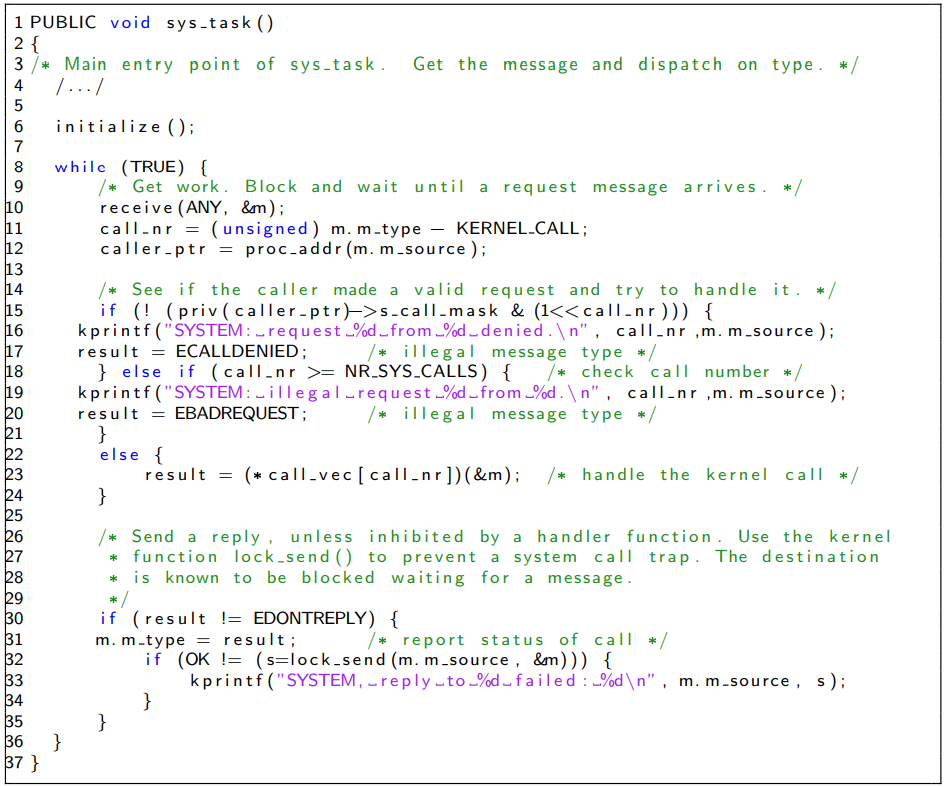
\includegraphics[scale=0.5]{sys-task.png}
\end{figure}
\begin{center}
  \textit{\small Ten krótki wycinek kodu został załączony za zachętą Osoby Serdecznie Zaangażowanej w Badania nad Kodem Minixa i z dedykacją dla niej}
\end{center}

\section{Organizacja pamięci}
\begin{table}[H]
  \centering
  \begin{tabular}{c|c}
    Rodzaj Pamięci & czas dostępu \\
    \hline
    Rejestry & 1-3 ns\\
    Level 1 Cache & 2-8 ns\\
    Level 2 Cache & 5-12 ns\\
    Memory & 10-60 ns\\
    Hard Disk & 3 000 000-10 000 000 ns
  \end{tabular}
  \caption{Hierarchia pamięci}
\end{table}
\subsection{Strategie alokacji}
Alokacja w większości systemów jest lazy, tzn. możemy sobie zażądać, ile chcemy pamięci, nawet więcej niż jest fizycznie dostępne, ale system de facto jej nam nie przydziela, dopóki jej nie dotkniemy.
\begin{itemize}
  \item First Fit - ani zły, ani dobry
  \item Next Fit - podobnie jak first fit
  \item Best Fit - wrzuca do najmniejszego w jakim się zmieści, niby brzmi fajnie, ale zostawia małe dziury, przez co potem ciężko coś wcisnąć
  \item Worst Fit - wrzuca na początku największego dostępnego fragmentu wolnego, fajny bo zostawia duże dziury
\end{itemize}
\subsection{Pamięć wirtualna}
Można tak gospodarować pamięcią RAM, żeby przydzielać procesom więcej pamięci niż jest fizycznej pamięci w komputerze. Nieużywane akurat dane przenosi się w inne miejsce (np. na dysk), a jeśli są potrzebne, to przywraca się je w jakimś dostępnym miejscu. Jeśli go zabraknie, to inne dane przenosi się na dysk. W UNIXowych systemach jest na to specjalnie wydzielona partycja na dysku (partycja ,,swap").
\subsection{Stronicowanie}
Obraz procesu i pamięć fizyczna dzielone są na strony, wszystkie o tym samym rozmiarze. Dla odróżnienia stron z obrazem procesu od stron pamięci fizycznej te drugie nazywamy ramkami. Strony mają rozmiar od kilku do kilkudziesięciu kilobajtów (zwykle 4kB w systemie 32-bitowym). Procesowi można przydzielić ramki w różnych miejscach, niekoniecznie obok siebie. Żeby odczytać zawartość strony, trzeba przetłumaczyć adres logiczny (numer strony, przesunięcie) na adres fizyczny. \\
Stronicowanie może być wielopoziomowe. W takim przypadku adres logiczny to pozycja tablicy w tablicy tablic, pozycja strony w tablicy stron, przesunięcie na stronie.
\begin{figure}[H]
  \centering
  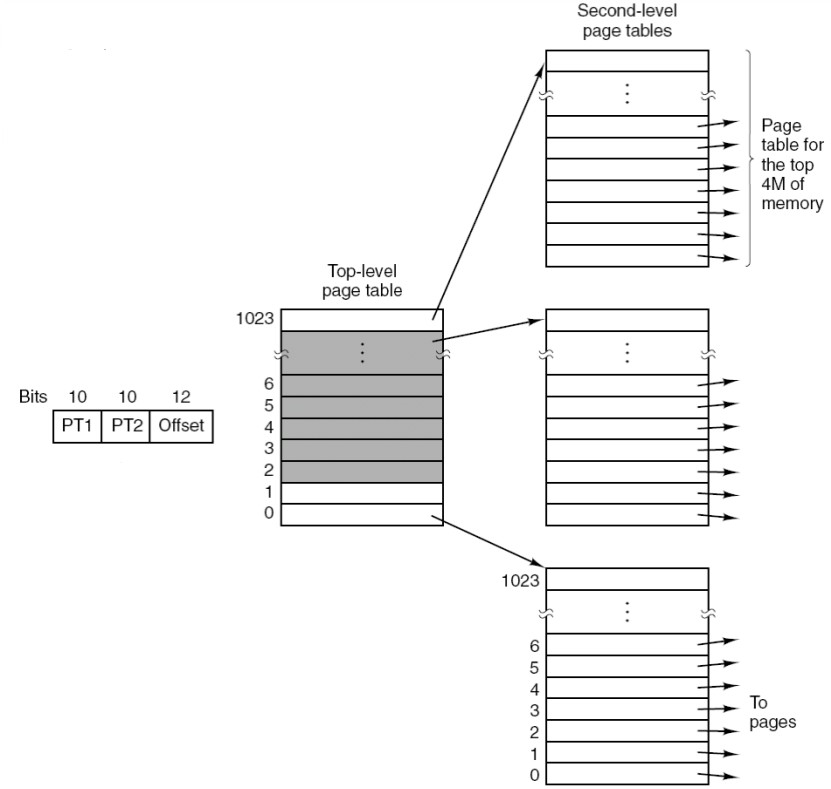
\includegraphics[scale=0.3]{stronicowanie.png}
\end{figure}
\begin{center}
  {\tiny https://lass.cs.umass.edu/~shenoy/courses/spring20/lectures/Lec11.pdf}
\end{center}
\subsubsection{Strategie ładowania stron}
\begin{itemize}
  \item Utopijna \textbf{strategia optymalna} - zastąp stronę, która będzie najpóźniej ładowana. Nie do zrealizowania online.
  \item \textbf{FIFO} - Wybierz ostatnio nieużywaną, mamy dodatkowe bity w tabeli stron, accessed i dirty. Bierzemy w kolejności (not referenced, not modified) $\rightarrow$ (not referenced, modified) $\rightarrow$ (referenced, not modified) $\rightarrow$ (referenced, modified), w ramach klasy losowo.
  \item \textbf{Second Chance / Clock PRA} - modyfikacja FIFO, usuwamy tylko, jeśli referenced = 0, wpp czyścimy referenced i przesuwamy na koniec kolejki. Zamiast kolejki lepiej używać bufora cyklicznego (clock).
  \item \textbf{Least recently used PRA} - zastąp stronę, która była użwana najdawniej. Implementacja wymaga wsparcia od hardware'u.
  \item \textbf{Not frequently used PRA} - po każdym przerwaniu kasuj bit referenced i zwiększaj licznik stronom, które mają ten bit ustawiony. Usuwaj te z najmniejszą wartością licznika.
  \item \textbf{Aging PRA} - po każdym przerwaniu dla każdej strony przesuń bity licznika o 1 w prawo, uzupełniając bitem referenced, po czym skasuj bit referenced. Usuwaj te z najmniejszą wartością licznika.
\subsubsection{Rozmiar strony}
Przyjęło się używać wzoru:
\begin{equation}
p = \sqrt{2se}
\end{equation}
Gdzie:\\
s - średni rozmiar procesu\\
e - rozmiar wiersza w tabeli stron\\
p - rozmiar strony\\\\
W większości systemów pracujących w 32 bitowej architekturze przyjmuje się:\\
s = 1MB, e = 8 \implies p = 4KB
\end{itemize}
\subsection{Segmentacja}
Segmenty mogą mieć różne długości, dlatego adres logiczny to numer segmentu (mapowany na adres bazowy, czyli adres początku segmentu) i długość danych do przeczytania. Podział na segmenty jest mniej więcej podziałem na logiczne części programu, więc niektóre z nich mogą być całkiem długie.
\subsection{W połączeniu}
Może być trudno znaleźć spójny fragment pamięci dla długiego segmentu, dlatego łączy się stronicowanie i segmentację i mamy segmenty składające się z ramek. Przesunięcie wewnątrz segmentu traktowane jest jako adres w pamięci stronicowanej (numer strony, przesunięcia na stronie). Zamiast adresu bazowego segmentu używany jest adres tablicy stron tego segmentu, w której można znaleźć numer ramki.
\subsection{Jak to działa w Linuxie?}
Jest tam więcej stronicowania, ponieważ łatwiej sobie z tym radzić, ale nie tylko stronicowanie.
\subsection{A w Minixie?}
Wersje Minixa starsze niż 3.1 nie miały stronicowania ani wirtualnej pamięci i cały proces musiał być załadowany do RAMu. Mogła się pojawić fragmentacja. Nowsze mają coś ze stronicowania i serwer VM, który jest oddzielony od PMa. Procesy były podzielone na segmenty.
\section{Drivery}
\textbf{\textit{Troszkę się zapędziliśmy, bo tego chyba nie przerabialiśmy, ale jest na slajdach. Sekcja niekompletna. Anyway, postanowiliśmy tego nie usuwać, a nóż komuś się przyda.}}\\\\
Drivery służą do interakcji z innymi urządzeniami.
Dzielą się na:\\\\
\textbf{Urządzenia blokowe} - mają swobodny dostęp do danych, czas dostępu do każdego fragmentu zbliżony, Dane zorganizowane w bloki, (np. CD/DVD-ROM)\\
\textbf{Urządzenia znakowe} - operują na ciągach znaków, dostęp sekwencyjny (np. klawiatura, mysz, modem)
\subsubsection{I/O port}
W architekturze x86 procesor ma do dyspozycji 216 8-bitowych portów. Porty mogą być grupowane dla zwiększenia transferu. Urządzenia mają oddzielną przestrzeń adresową.
\subsubsection{Memory mapped I/O}
Można też zmapować rejestry urządzeń do przestrzeni adresowej pamięci procesora. Dostęp jak do pamięci (np. MOV).
\subsubsection{Spooling}
Tryb realizowania operacji wejścia-wyjścia w odniesieniu do urządzeń o dostępie wyłącznym. Cała zawartość strumienia jest buforowana zanim zostanie przesłana w miejsce docelowe.

\chapter{Rozwiązania egzaminów}
\section{Egzamin 2013/2014}
\textbf{Zadanie 1} \\
konieczność wielokrotnego przełączania procesów spowodowana dużą liczbą wywołań systemowych \\\\
\textbf{Zadanie 2} \\
Mamy takie zależności (x $\rightarrow$ y ozn x pojawi się przed y): \\
c1 $\rightarrow$ p1, c2 $\rightarrow$ p2, p1 $\rightarrow$ p2 \\
1. nie \\
2. nie \\
3. tak \\
4. tak
\\\\
\textbf{Zadanie 3} \\
mniejszy koszt przełączania procesora pomiędzy wątkami niż pomiędzy procesami \\\\
\textbf{Zadanie 4} \\
1. micro \\
2. żaden – w mikrojądrze tylko jądro pracuje w trybie uprzywilejowanym, a w systemie monolitycznym procesy mogą wykonywać jedynie kod jądra w uprzywilejowaniu \\
3. mono – procesy same przełączają się na bycie driverami, bo nie ma serwerów \\
4. mono – na przykład żeby wykonać syscall \\\\
\textbf{Zadanie 5} \\
1. tak
2. nie
3. nie
4. nie \\\\
\textbf{Zadanie 6} \\
1. nie \\
2. tak – kiedy procesy równolegle zawieszą się na semaforach AB oraz BA \\
3. nie – przykład notify \\
4. tak – przykład send, receive \\\\
\textbf{Zadanie 7} \\
1. pag \\
2. seg, pag \\
3. seg, pag \\
4. pag \\
5. seg \\
6. pag \\
7. pag \\\\
\textbf{Zadanie 8} \\
1. nie \\
2. tak \\
3. tak \\
4. tak \\\\
\textbf{Zadanie 9} \\
1. tak \\
2. tak \\
3. 
4. nie \\\\

\section{Egzamin 2014/2015}
\textbf{Zadanie 1} \\
5 \\\\
\textbf{Zadanie 2} \\
Jeśli otwieramy pipe O\_RDONLY lub O\_WRONLY i po drugiej stronie nikogo nie ma. \\\\
\textbf{Zadanie 3} \\
Jeśli write jest przerwany, to zwróci rozmiar tego, co udało się zapisać lub -1, jeśli nic. \\\\
\textbf{Zadanie 4} \\
Sygnały się nie stackują. \\\\
\textbf{Zadanie 5} \\
select \\\\
\textbf{Zadanie 6} \\
send \\
Nie jest buforowany, więc jest blokujący. \\
Przenosi dane. \\
notify \\
Jest buforowany i nieblokujący. \\
Powiadomienie nie jest koniecznie od konkretnego procesu. \\
Nie przenosi danych. \\\\
\textbf{Zadanie 7} \\
3.1.0: FS, Disc Driver, System Task \\
3.2.2: VFS, ???, Disc Driver, System Task \\\\
\textbf{Zadanie 8} \\
throughput - ? \\
turnaround time - zmniejszy (mniej czasu traconego na zmianę kontekstu) \\
response time - zwiększy (dłuższy czas czekania w kolejce) \\\\
\textbf{Zadanie 9} \\
Prawdopodobnie porty \\\\
\textbf{Zadanie 10} \\
Część pamięci może być przeniesiona na dysk bez wiedzy procesu. \\\\

\section{Egzamin 2015/2016}
\textbf{Zadanie 1} \\
i-node, tablica tablic, tablica wskaźników, node z plikiem \\\\
\textbf{Zadanie 2} \\
Jeśli plik jest odpowiednio duży, to cat zapełni cały pipe i dziecko zawiesi się na blokującym write. W tym samym czasie rodzic czeka na jego zakończenie i takczekąją, i czekają.nikt nie czyta z pipe’a. Jeśli plik jest mały, to dziecko nie zablo-kuje się przy pisaniu i zakończy, więc rodzic będzie mógł odnotować to i przejśćdo dalszej pracy. \\\\
\textbf{Zadanie 3} \\
Signaled \\
Dziecko najprawdopodobniej zostanie zakończone sygnałem podczas wykonywania cat. Handlery nie przenoszą się przez exec. \\\\
\textbf{Zadanie 4} \\
Pod rm wywołany jest unlink, ale w systemie mogło być więcej linków do tego pliku. \\\\
\textbf{Zadanie 5} \\
W kernelu jest tabela, w której zapisane są uprawnienia. Wszystkie procesy użytkownika mają jeden wspólny rekord, a pozostałe procesy oddzielne. Są tam zapisane maski kernel calli, które dany proces może wywoływać. \\\\
\textbf{Zadanie 6} \\
Jeśli proces nie wykorzystał w pełni swojego kwantu czasu, to po odblokowaniu zostaje dodany
na początek swojej kolejki. Dodatkowo procesy, które dwa razy z rzędu dostały czas procesora i wykorzystały swój kwant są degradowane. \\\\
\textbf{Zadanie 7} \\
send \\
Nie jest buforowany, więc jest blokujący. \\
Przenosi dane. \\
notify \\
Jest buforowany i nieblokujący. \\
Powiadomienie nie jest koniecznie od konkretnego procesu. \\
Nie przenosi danych. \\\\
\textbf{Zadanie 8} \\
nie? \\
tak \\
tak \\
tak? \\
nie \\
nie \\
nie \\\\
\textbf{Zadanie 9} \\
fx, fy, fz \\
fz, fx, fy \\\\
\textbf{Zadanie 10} \\
Tak działa cache'owanie. \\\\

\section{Egzamin 2016/2017}
\textbf{Zadanie 1} \\
Write nie jest buforowany, więc zapisanie każdego znaku wymaga osobnego syscalla. \\\\
\textbf{Zadanie 2} \\
Jeśli plik jest odpowiednio duży, to cat zapełni cały pipe i dziecko zawiesi się na blokującym write. W tym samym czasie rodzic czeka na jego zakończenie i tak czekąją, i czekają.nikt nie czyta z pipe'a. Jeśli plik jest mały, to dziecko nie zablokuje się przy pisaniu i zakończy, więc rodzic będzie mógł odnotować to i przejść do dalszej pracy. \\\\
\textbf{Zadanie 3} \\
To procesy, które czekają na osierocone procesy, żeby nie stały się zombie, kiedy rodzic  już sie zakończył i nie odnotował ich stanu. Liczba 1613 to reaper, a 1 na Minixie to init. \\\\
\textbf{Zadanie 4} \\
Jeśli wyczerpał swój kwant, trafi na koniec, a jeśli zostało mu jeszcze troszkę czasu, to na początek. \\\\
\textbf{Zadanie 5} \\
komunikacja z (fizycznym) dyskiem \\
message-passing pomiędzy driverem a procesem \\\\
\textbf{Zadanie 6} \\
Można wykorzystać funkcję select albo poll, żeby dowiedzieć się, że któryś z pipe’ów jest gotowy na wpisanie do niego danych. \\\\
\textbf{Zadanie 7} \\
Handler obsługujący przerwania od klawiatury dodaje hdd do kolejki schedulera. \\\\
\textbf{Zadanie 8} \\
Do tego służą przerwania zegarowe, które budzą scheduler i pozwalają mu robić porządki. \\\\
\textbf{Zadanie 9} \\
Może się tak stać, jeśli strona w pamięci jest dwukrotnie zmapowana w przestrzeni procesu, czyli arr[42] w pamięci fizycznej odpowiada dwóm miejscom w pamięci wirtualnej. Można to zrobić funkcją mmap. \\\\
\textbf{Zadanie 10} \\
To sposób organizacje miejsca na dysku. Polega na tym, że dane upychane są w dostępnych miejscach pamięci, które mogą być zupełnie porozrzucane, ale co jakiś czas reorganizujemy dane tak, żeby fragmenty pliku były względnie blisko siebie. Pozwala to zmniejszyć czas odczytu. \\\\

\section{Egzamin 2017/2018}
\textbf{Zadanie 1} \\
Możliwe odpowiedzi:
1. read może wczytać fragmentaryczne dane
2. może pojawić się sygnał i błąd EINTR
3. exec może się nie udać i dziecko się zapętli
Program dostaje zupełnie nieprzewidywalny argument. \\\\
\textbf{Zadanie 2} \\
Chodzi o to, że handlery nie zachowują się przy execu, a maska tak (SIG\_IGN działa jak ustawianie maski). Dlatego proces dziecka będzie miał blokowane SIGUSR2 i SIGINT, ale SIGUSR1 nie. Program wypisze 1 kropkę, bo SIGUSR1 zakończy proces potomny. \\\\
\textbf{Zadanie 3} \\
To procesy, które czekają na osierocone procesy, żeby nie stały się zombie, kiedy rodzic  już sie zakończył i nie odnotował ich stanu. Liczba 1613 to reaper, a 1 na Minixie to init. \\\\
\textbf{Zadanie 4} \\
1. utworzenie nowego wątku \\
2. zablokowanie procesu \\
3. zakończenie procesu \\
4. wyczerpanie kwantu \\
5. przerwanie zegarowe \\
6. przerwanie IO \\\\
\textbf{Zadanie 5} \\
? \\\\
\textbf{Zadanie 6} \\
1. wspóldzielona pamięć \\
2. porty IO \\
3. przerwania \\\\
\textbf{Zadanie 7} \\
Zalety: \\
1. Pamięć nie jest rezerwowana na zapas - mniejszy narzut. \\
2. Pojedyńcza operacja jest szybsza. \\
3. Procesy uruchamiają się szybciej. \\
Wady: \\
1. Opóźnienie przy pierwszym dostępie do pamięci związane z obsługą page faulta przez
system operacyjny. \\
2. Bardziej złożona obsługa. \\
3. Duża częstotliwość występowania page faultów \\\\
\textbf{Zadanie 8} \\
System utworzy stos dla procesu, na którym na początku jest są dane z programu. Na szczycie zostaną ułożone argumenty, a potem uruchomiony proces. \\\\
\textbf{Zadanie 9} \\
Może się tak stać, jeśli strona w pamięci jest dwukrotnie zmapowana w przestrzeni procesu, czyli arr[42] w pamięci fizycznej odpowiada dwóm miejscom w pamięci wirtualnej. Można to zrobić funkcją mmap. \\\\
\textbf{Zadanie 10} \\
Mógł być wykorzystywany przez handler. \\
Mógły być tam ułożone informacje o procesie. \\\\

\section{Egzamin 2018/2019}
\textbf{Zadanie 1} \\
14 \\\\
\textbf{Zadanie 2} \\
Select poinformuje o gotowości do odczytu zbyt wcześnie, ponieważ odczyt z pipe'a zamkniętego po drugiej stronie jest traktowany jako otwarty. Więc po zamknięciu pipe'a przez producenta powstaje aktywne czekanie. \\\\
\textbf{Zadanie 3} \\
Jeśli przez 3 sekundy nie pojawi się input, to przyjdzie alarm, który nie jest obsługiwany i proces się zakończy. \\\\
\textbf{Zadanie 4} \\
To procesy, które czekają na osierocone procesy, żeby nie stały się zombie, kiedy rodzic  już sie zakończył i nie odnotował ich stanu. Liczba 1613 to reaper, a 1 na Minixie to init. \\\\
\textbf{Zadanie 5} \\
Użycie printf i exit w handlerze jest ryzykowne - co jeśli się nie powiodą? On ne fait pas des choses comme ça \\\\
\textbf{Zadanie 6} \\
Zwykły użytkownik nie może wywołać sys\_fork, bo komunikację z kernelem wykonują serwery i drivery (np. PM czy VFS). Dla użytkowników przeznaczone są zwykłe syscalle, które komunikują się przez serwery. \\\\
\textbf{Zadanie 7} \\
1. powstanie nowego wątku \\
2. wyczerpanie kwantu \\
3. doczekanie się odpowiedzi lub dostępu do zasobów \\\\
\textbf{Zadanie 8} \\
Driver chce doczytać bliższe sektory na dysku, by przyśpieszyć przyszłe dostępy do pamięci w tych okolicach (pewnie też będą niedługo potrzebne - założenie często słuszne). \\\\
\textbf{Zadanie 9} \\
Dostęp do początku pliku jest od razu, a żeby dostać się do końca trzeba przeczytać pośrednie bloki. Asymptotycznie czas jest logarytmiczny (mamy drzewo i-nodów), praktycznie stały rzędu 3. \\\\
\textbf{Zadanie 10} \\
page fault frequency mówi jak często programy odwołują się do pamięci obiecanej przez system, ale nie przydzielonej. Jeśli program nigdy nie odwołał się albo nie odwoływał przez dłuższy czas do jakiegoś miejsca, to może być przeniesione na dysk i kiedy nastąpi page fault, to trzeba je ściągnąć z powrotem do pamięci podręcznej. Jeśli pojawia się bardzo dużo page faultów, to może tak być, że system obiecał zbyt wielu zbyt wiele i brakuje pamięci pod ręką, więc trzeba swapnąć któryś proces na dysk. \\\\
\textbf{Zadanie 10} \\
Printf jest buforowany, a dzieciom kopiuje się bufor rodzica, w którym już są kropki.

\section{Egzamin 2019/2020}
\textbf{Zadanie 1} \\
Wykorzystamy oznaczenia
p – pid programu \\
q – pid dziecka \\
r – pid reapera \\
x – pid rodzica programu \\
,,Zwykle" (wszystko się powiedzie, bufor się nie skopiuje) mamy tylko trzy opcje: \\
Dziecko pracuje pierwsze: \\
p x \\
0 q p \\
q p x \\\\
Rodzic pracuje pierwszy, ale kończy się później niż dziecko: \\
p x \\
q p x \\
0 q p \\\\
Rodzic pracuje pierwszy i kończy się wcześniej niż dziecko: \\
p x \\
q p x \\
0 q r \\\\
\textbf{Zadanie 2} \\
dup \\
Kopiuje deskryptor, mamy nowy odnośnik do pliku \\
Miejsce z którego czytamy to to, w którym skończyliśmy ostatni odczyt \\
open \\
Tworzy nowe open file description \\
Odczyt zaczyna się na początku pliku \\\\
\textbf{Zadanie 3} \\
Alarmy dotyczą tylko procesu, który o niego prosił i przenoszą się przez exec. \\
Dziecko wypisze dwie kropki w warunku i dwie tuż przed wyjściem. Zależnie od czasu alarmu i spanka rodzic dopisze swoją trzecią kropkę lub nie. \\\\
\textbf{Zadanie 4} \\
Sygnały się nie kolejkują, więc handler może wywołać się jeden raz i powstaną zombie. \\\\
\textbf{Zadanie 5} \\
exit w handlerze, dobranoc (jeśli koniecznie (dalece niezalecane) chcemy wyleźć z programu w
handlerze to używamy \_exit) \\\\
\textbf{Zadanie 6} \\
Jeśli proces nie wykorzystał w pełni swojego kwantu czasu, to po odblokowaniu zostaje dodany
na początek swojej kolejki. Dodatkowo procesy, które dwa razy z rzędu dostały czas procesora i wykorzystały swój kwant są degradowane. \\\\
\textbf{Zadanie 7} \\
1. komunikacja między procesami \\
2. obsługa urządzeń oraz przerwań \\
3. obsługa IO \\
4. obsługa zegara \\\\
\textbf{Zadanie 8} \\
open musi znaleźć odpowiedni i-node (długość ścieżki = liczba katalogów po drodze). \\
lseek tylko zmienia ustawienie w odpowiedniej tablicy \\
read czyta z dysku parę sektorów \\\\
\textbf{Zadanie 9} \\
Stara się podnosić i restartuje serwery, kiedy się popsują \\
Przechowuje i udziela informacji o endpointach serwerów \\\\
\textbf{Zadanie 10} \\
page fault frequency mówi jak często programy odwołują się do pamięci obiecanej przez system, ale nie przydzielonej. Jeśli program nigdy nie odwołał się albo nie odwoływał przez dłuższy czas do jakiegoś miejsca, to może być przeniesione na dysk i kiedy nastąpi page fault, to trzeba je ściągnąć z powrotem do pamięci podręcznej. Jeśli pojawia się bardzo dużo page faultów, to może tak być, że system obiecał zbyt wielu zbyt wiele i brakuje pamięci pod ręką, więc trzeba swapnąć któryś proces na dysk. \\\\

\section{Egzamin 2020/2021}
\textbf{Zadanie 1} \\
Rodzi zrobi fork, wywoła main, wypisze kropkę i zakończy pracę, ponieważ f będzie równe 1.
Z kolei dziecko wywoła ten sam program, ale z użyciem execa, więc f z powrotem będzie równe 0 i tak zaobserwujemy potencjalnie nieskończenie wiele kropek. Chyba że któryś fork po drodze się nie uda, wtedy program się nie zapętli. \\\\
\textbf{Zadanie 2} \\
.. \\
.. \\
Pierwsze dwie kropki wypisze exec i proces się zakończy. Kolejne dwie zostaną wypisane w nahlerze dziecka i rodzica po otrzymaniu SIGUSR1. Na koniec SIGUSR2 pozbędzie się wszystkich procesów. \\\\
\textbf{Zadanie 3} \\
FD\_CLOEXEC gwawrantuje, że deskryptor będzie zamknięty przed exec. Dlatego wypisanie się nie uda, bo stdout zostanie zamknięty. \\\\
\textbf{Zadanie 4} \\
TICTIC \\
Tryb O\_RDWR oznacza, że proces ma otwarty i koniec do pisania i do czytania, a nie da się odróżnić, kto co napisał. Dziecko zapisze TIC, po czym je przeczyta, kiedy rodzic będzie spał i zostawi pusty pipe. Przed wyjście wypisze TICTIC. Rodzic nie będzie miał nic do czytania, ale ponieważ sam trzyma koniec do pisania, to read będzie blokujący i tak się zawiesi w oczekiwaniu. \\\\
\textbf{Zadanie 5} \\
Procesy dzieci bedą się kończyć prawie równo, a sygnały się nie kolejkują. Przybędzie parę zombie. \\\\
\textbf{Zadanie 6} \\
dirty - czy była modyfikowana i trzeba to będzie zapisać na dysku \\
accessed - czy była niedawno odczytywane, bit jest co jakiś czas zerowany przez system \\\\
\textbf{Zadanie 7} \\
HARD\_INT oznacza Hardware Interrupt. W tym przypadku jako przerwanie systemowe pochodzą
pewnie od urządzenia pełniącego rolę zegara i oznaczają, że przesunąć przesunąć
czas o kolejny tick. \\\\
\textbf{Zadanie 8} \\
Pierwszy odczyt jest powolny bo wymaga sięgnięcia na dysk, a fragmenty pliku mogą nie być w spójnym fragmencie pamięci. Linux cache’uje sobie w RAMie zawartość tego pliku, dzięki czemu kolejne odczyty są szybciutkie. \\\\
\textbf{Zadanie 9} \\
VFS ma stały endpoint, a IPC nie, więc za każdym razem trzeba pytać RSa który proces to IPC. \\\\
\textbf{Zadanie 10} \\
Jeśli wszystko byłoby przekazywane przez wskaźnik to proces, który odbiera wiadomość musiałby
sam odczytać/skopiować napis spod wskaźnika, który wskazuje na pamięć innego procesu. Taki mechanizm jest bardziej kosztowny niż po prostu odczytanie z wiadomości, która należy do odbiorcy. \\\\

\section{Egzamin 2021/2022}
\textbf{Zadanie 1} \\
1. AB \\
2. ABB \\
3. ABC \\ 
4. ABBC \\
5. ABBCC \\
6. ABCB \\
7. ABCBC \\
Na początku na pewno pojawią się litey A i B. Przy czym B może się pojawić dwa razy. Litera C pojawi się maksymalnie 2 razy (zanim dzieci obu równoległych procesów zabiją całą grupę poprzez kill 0). Jeśli form się nie uda, to kill -1 zakończy wszystkie procesy (w tym wypadku dotrze do tej samej grupy co kill 0). \\\\
\textbf{Zadanie 2} \\
\begin{verbatim}
  int main() {
    int fd[2];
    pipe(fd);
    while(1) {
      write(fd[1], "A", 1);
    }
  } 
\end{verbatim}
Kiedy w buforze skończy się miejsce, to write się zablokuje. \\\\
\textbf{Zadanie 3} \\
FD\_CLOEXEC gwawrantuje, że deskryptor będzie zamknięty przed exec. Dlatego wypisanie się nie uda, bo stdout zostanie zamknięty. \\\\
\textbf{Zadanie 4} \\
Problem polega na tym, że deskryptory są kopiowane (dup2), ale nie są nigdzie zamykane, a jest górne ograniczenie na ich liczbę (16 w Linuxie), więc po pewnym czasie program zakończy się z błędem. Trzeba by zamykać deskryptor po skopiowaniu. \\\\
\textbf{Zadanie 5} \\
W kernelu każdy deskryptor reprezentowany jest przez strukturę struct\_fd, która przechowuje wskaźnik do open file description. W ofd sa takie informacje jak tryb otwarcia, flagi, pozycja kursora, etc. Wiele fd może wskazywać na to samo ofd, kazdy fd może wskazywać tylko na jeden ofd. Dla ofd jest co najmniej kilka flag, np O\_APPEND lub O\_TRUNC, a dla fd tylko jedna nam znana, FD\_CLOEXEC. \\\\
\textbf{Zadanie 6} \\
ready – w oczekiwaniu na przydzielenie czasu procesora \\
blocked – w oczekiwaniu na zdarzenie, np. odpowiedź na wiadomość lub zwolnienie zasobów \\
swapped – zatrzymany, ze stanem zapisanym na dysku twardym (bo zabrakło pamięci)
zombie – zakończony, co nie zostało odnotowane przez rodzica \\\\
\textbf{Zadanie 7} \\
To znaczy, że najpewniej brakuje pamięci, więc trzeba swapować jakiś proces na dysk. \\\\
\textbf{Zadanie 8} \\
Lepiej pozwolić najpierw pracować dziecku, ponieważ nie trzeba kopiować pamięci, dopóki któryś z procesów (dziecko lub rodzic), nie zaczną po niej pisać. Jest duże prawdopodobieństwo, że dziecko wywoła execa, więc i tak trzeba będzie zorganizować dla niego pamięć. Gdyby rodzic zaczął pracę jako pierwszy, pewnie szybko przeszedłby do pisania po pamięci i dwukrotnie trzeba by organizować pamięć dziecka - skopiować tę od rodzica i przygotować nową do exec. \\\\
\textbf{Zadanie 9} \\
Stara się podnosić i restartuje serwery, kiedy się popsują \\
Przechowuje i udziela informacji o endpointach serwerów \\\\
\textbf{Zadanie 10} \\
Strony będą miały adresy od 4095 do 8000 i trochę, a kolejna do 12000 i trochę, więc x znajdzie się na jednej stronie a y i z razem na innej. Strony mogą być przechowywane w pamięci w dowolnej kolejności, stąd są dwa możliwe scenariusze: \\
x y z \\
y z x \\\\

\section{Egzamin 2022/2023}
\textbf{Zadanie 1} \\
3 \\
setsid tworzy nową, niezależną grupę procesów. Powstaną trzy grupy, a w każdej tylko najszybszy z procesów wypisze kropkę, bo potem zakończy pracę wszystkich w grupie. \\\\
\textbf{Zadanie 2} \\
a c d \\
Printf jest buforowany \_exit kończy program bez wcześniejszego opróżniania buforów. \\\\
\textbf{Zadanie 3} \\
Kod biblioteki jest ładowany dynamicznie, czyli jest jakby współdzielony. Dzięki temu zajmuje mniej miejsca i można łatwo uaktualniać go dla wszystkich procesów, ale z drugiej strony trzeba zadbać o jego bezpieczeństwo. \\\\
\textbf{Zadanie 4} \\
SIGKILL oraz SIGSTOP \\\\
\textbf{Zadanie 5} \\
To są procesy zombie. \\\\
\textbf{Zadanie 6} \\
Nie ustawiamy ani act.sa\_mask, ani act.sa\_flags i nie wiadomo, jak wyglądają, więc nie można oczekiwać, że zachowanie programu będzie zdefiniowane. \\\\
\textbf{Zadanie 7} \\
Jeśli proces nie wykorzystał w pełni swojego kwantu czasu, to po odblokowaniu zostaje dodany
na początek swojej kolejki. Dodatkowo procesy, które dwa razy z rzędu dostały czas procesora i wykorzystały swój kwant są degradowane. \\\\
\textbf{Zadanie 8} \\
Prawdopodobnie plik jest pusty poza jakimś znakiem na odległej pozycji. I-nody nie przechowują pustej zawartości, więc zajmują mniej miejsca niż rozmiar pliku. \\\\
\textbf{Zadanie 9} \\
Pamięć wirtualna ma oddzielne adresowanie dla każdego procesu, więc potrzebne są identyfikatory procesów, żeby określić fizyczne adresy.\\\\
\textbf{Zadanie 10} \\
System cache’uje plik. Pierwsze użycie czyta z dysku, kolejne dwa czytają z RAMu. \\\\

\begin{thebibliography}{3}
\bibitem{tanenbaum}
Operating Systems: Design and Implementation - Andrew S. Tanenbaum, Albert S. Woodhull
\bibitem{wikipl}
\href{https://pl.wikipedia.org/}{pl.wikipedia.org}, zbyt dużo, żeby linkować pojedyńczo
\bibitem{wikieng}
\href{https://en.wikipedia.org/}{en.wikipedia.org}, zbyt dużo, żeby linkować pojedyńczo
\bibitem{jkozik}
Wykłady Prof. Jakuba Kozika z Systemów Operacyjnych na TCS UJ.
\bibitem{man}
\href{https://man7.org/linux/}{man7.org}
\bibitem{mimuw}
\href{https://students.mimuw.edu.pl/~mk371127/documents/7/przeczytaj_mnie.html}{Strona o systemach operacyjnych mimuw}
\bibitem{umass}
\href{https://lass.cs.umass.edu/~shenoy/courses/spring20/lectures/Lec11.pdf}{Materiały Uniwersytetu Massachusetts}
\bibitem{SO}
SO-Suffering, materiały TCSu
\bibitem{JH}
\href{https://matematykawmiiuj.wordpress.com/systemy-operacyjne/}{Materiały opracowane przez Weronikę Lorenczyk, Wojciecha Węgrzynka i Jędrzeja Hodora}
\end{thebibliography}
\end{document}
